\chapter{提案手法の統合}

\section{提案手法}

これまでに説明してきた手法の中で,検索性能の向上に有効な結果を示したものを統合し,検索精度の更なる向上を図る.検索性能の向上に有効な結果を示したものとして,論文の利用・Kaldiを用いた検索文書の利用・キャッシュモデル・前後の部分文書の情報を加味の手法があり,これらを統合し,検索精度の変化を分析する.

\subsection{実験条件}
実験条件を表\ref{t_ex_patern}に示す.

\begin{table}[h]
    \centering
    \caption{実験条件}
    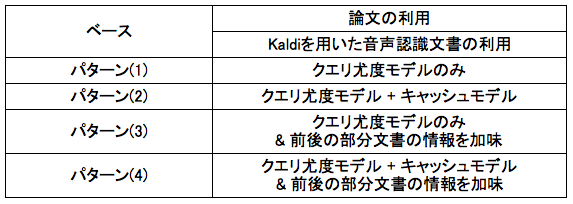
\includegraphics[width=7cm]{./image/t_ex_patern.png}
    \label{t_ex_patern}
\end{table}

実験は,表\ref{t_condition1}と同様に,NTCIR12 SpokenQuery\&Doc Formal-run の SQSCR SGS retrieval条件で行った.
基本的に,論文の利用とKaldiを用いた検索文書を用い,パターン(1) クエリ尤度モデルのみ, パターン(2) キャッシュモデルの2つのパターンについて,変化させたときのMAP値を算出する.
また,2つのパターンのそれぞれに対し,前後の部分文書の情報を加味をした4パターンについて比較,分析した.

% TODO: パラメータの説明もメモしといた方が良い